\documentclass[a4paper,12pt]{report}
\usepackage{graphicx}
\usepackage{titlesec}
\titleformat{\chapter}{}{}{0em}{\bf\LARGE}
\usepackage[utf8]{inputenc}
% Title Page
\title{Middle East Technical University\\Department of Physics\\PHYS222 Optics and Waves Laboratory\\\textbf{Experiment OW-9\\Reflection\\Laboratory Report}}

\author{Oğuzhan ÖZCAN\\1852334\\\\Partner: İnci SAİM\\\\Teaching Assistant: Hikmet ÖZŞAHİN}


\begin{document}
\maketitle
\tableofcontents
\listoffigures
\listoftables
\chapter{Theory}
When a beam of light strikes to a transparent surface such as a sheet of glass, the wave faces to a vast array of atoms whose are closely seperated. As we mentioned in previous experiments, visible light spectrum is between approximately 370 and 700 nm. On the other hand, atoms and their seperations is $\theta$ 0.2 nm which means seperation between atom thousands times of smaller than light ray. When a beam of light strikes such an interference, some light is always scattered backward. In optics, this phonemena known as \textit{reflection.}
\begin{figure}[h!]
\centering
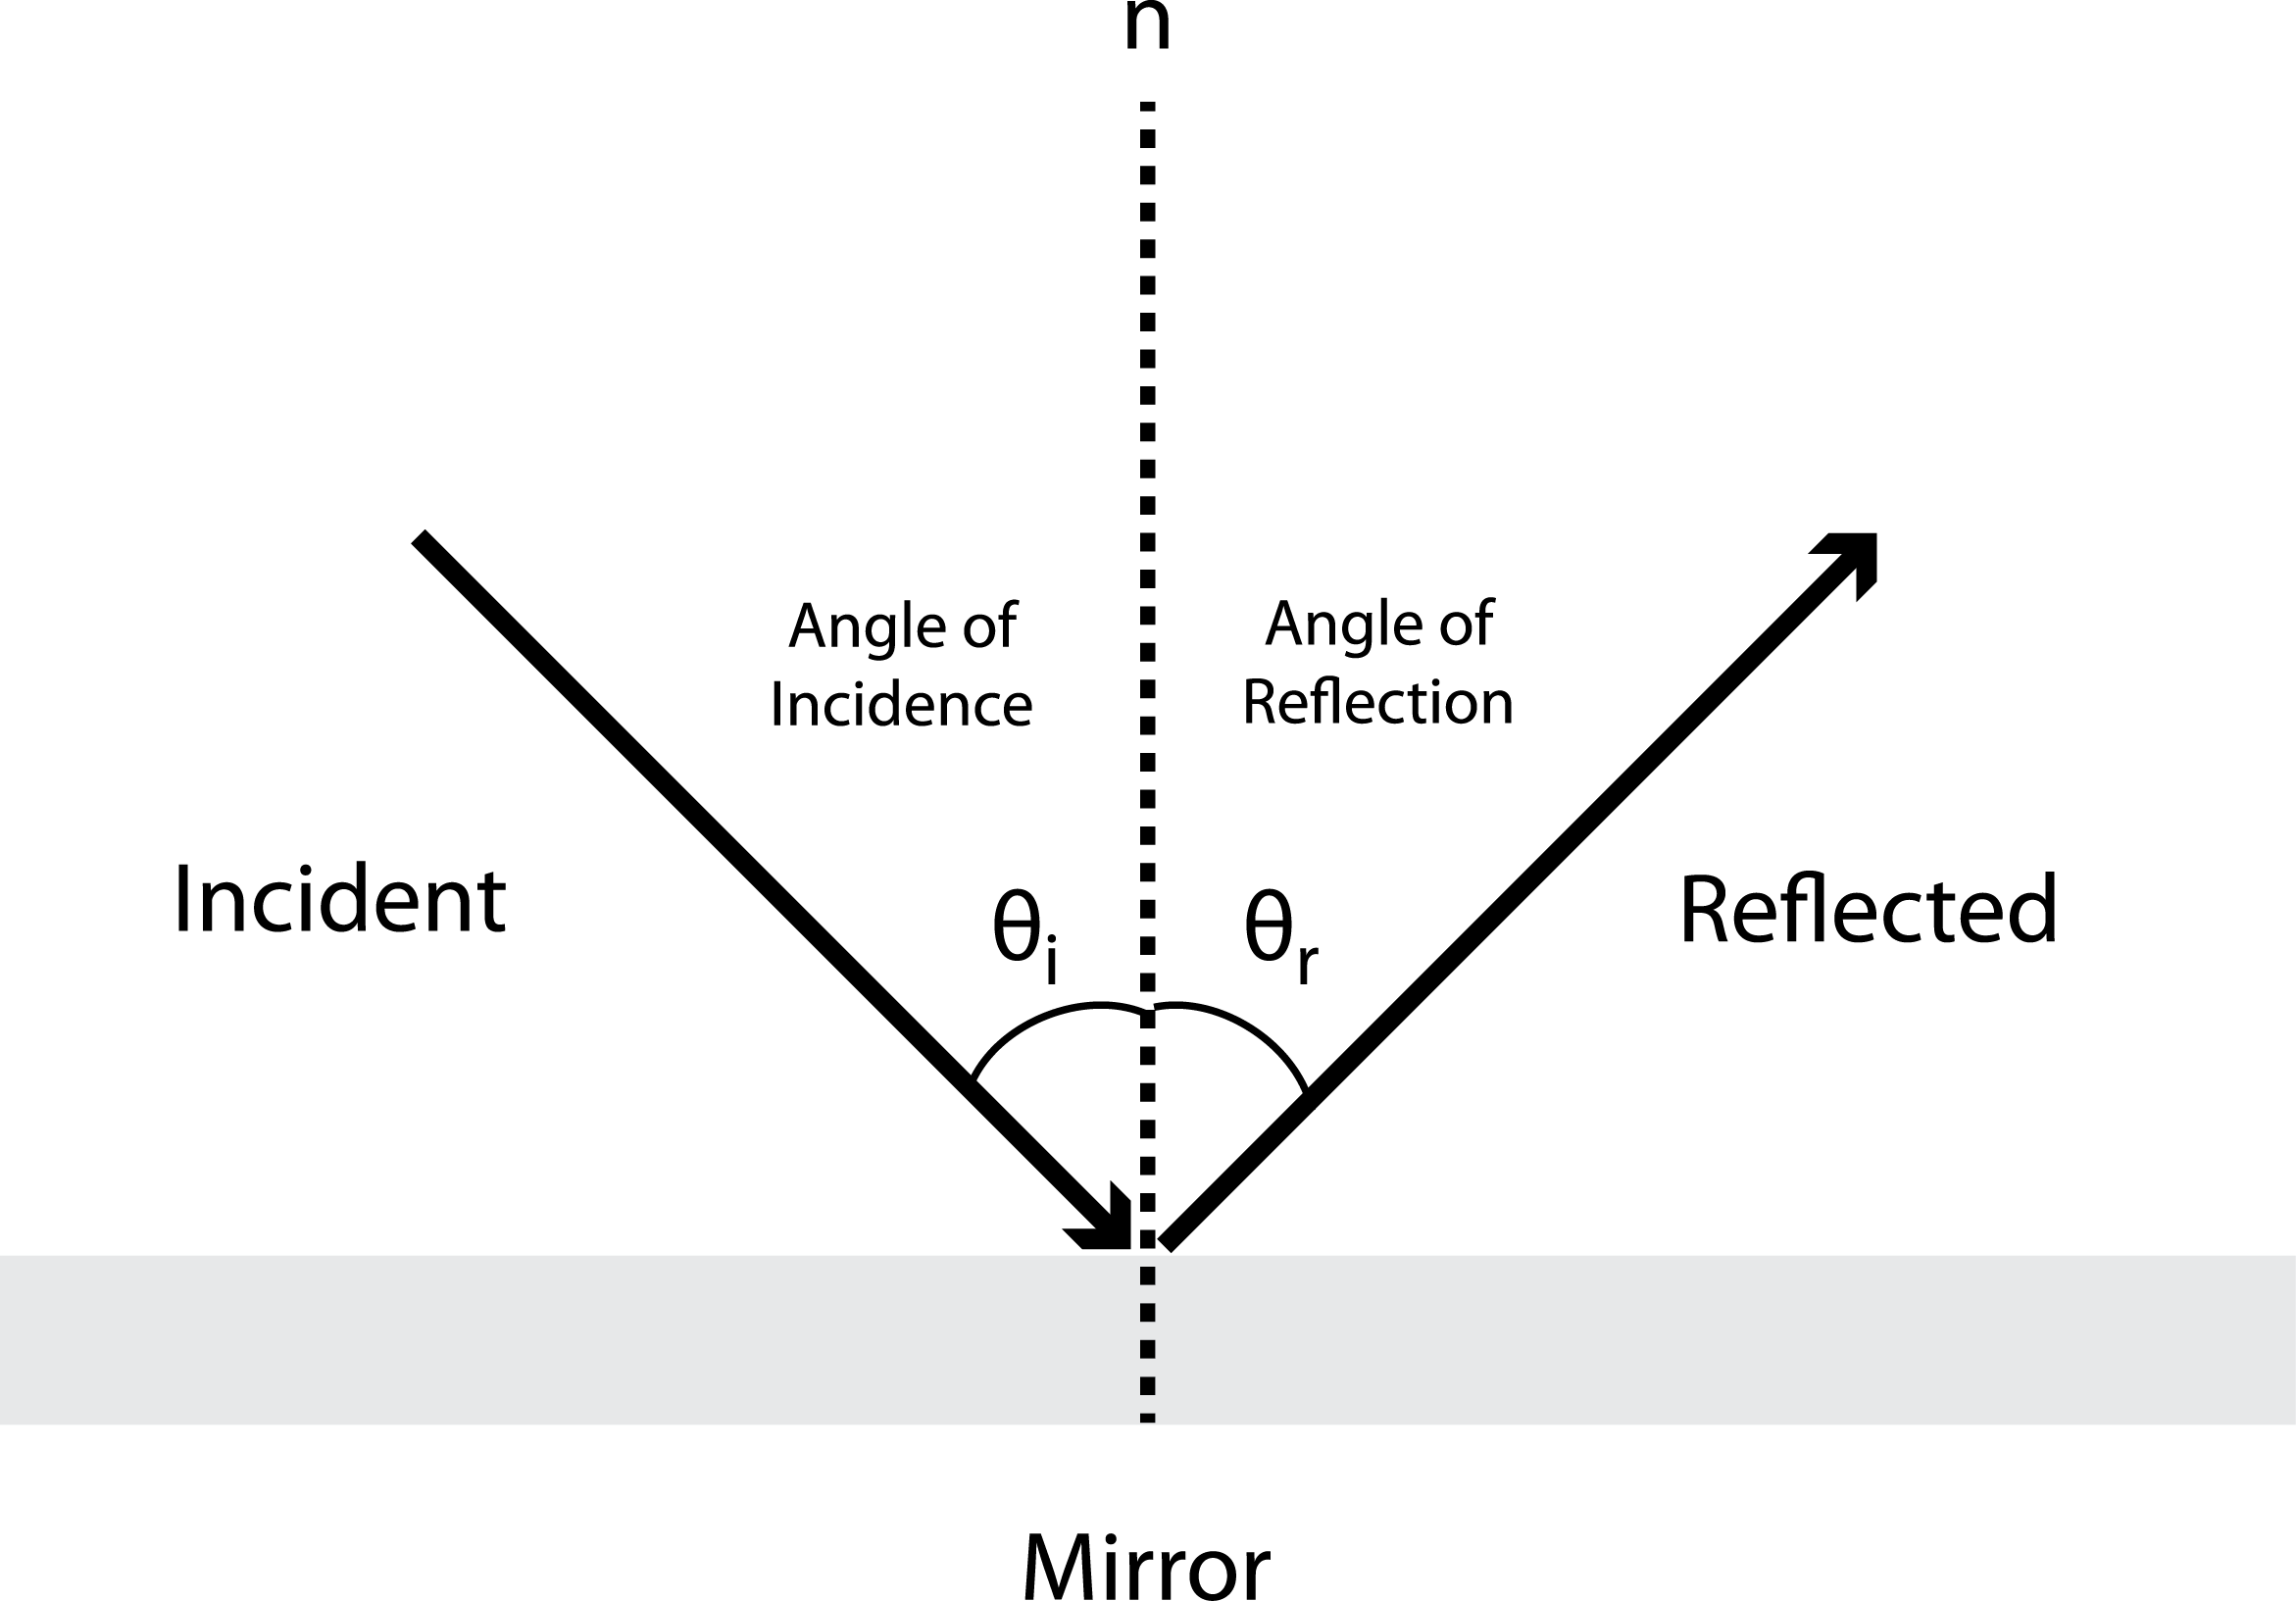
\includegraphics[width=0.7\linewidth, height=0.35\textheight]{Untitled-2}
\caption{Reflection from a mirror}
\label{fig:Untitled-2}
\end{figure}

In the simplest case, the angle of ray which is strikes to mirror or plane is exactly equal to angle which belongs to reflected ray. Before measure the angle of incidence and angle of reflection, we have to put a perpendicular line to related surface. In the Figure 1.1, this line can be seen as \textit{n}. Generally, this line called as \textit{normal.}If angle of incidence $\phi$ increases then angle of reflection also increases in the exactly same amount. That is why we can say that 
\begin{center}
	angle of incidence = angle of reflection
\end{center}
Above equation is the first part of the \textit{Law of Reflection}. Actually, this equation firstly appeared in the Euclid's book \textit{Catoptrics} [1]. So, we can write that
\begin{center}
	$\theta=\theta^{\prime}$ or $\theta_{i}=\theta_{r}$
\end{center}
We say that if the angle of incidence $\theta_{i}$ is 0$^{\circ}$, this beam is normally incident which means mirror reflects the beam back on itself and besides angle of reflection $\theta_{r}$ is also 0$^{\circ}$. These rules can also be obtained from the application of boundary conditions for electromagnetic waves [2].
\begin{figure}[h!]
\centering
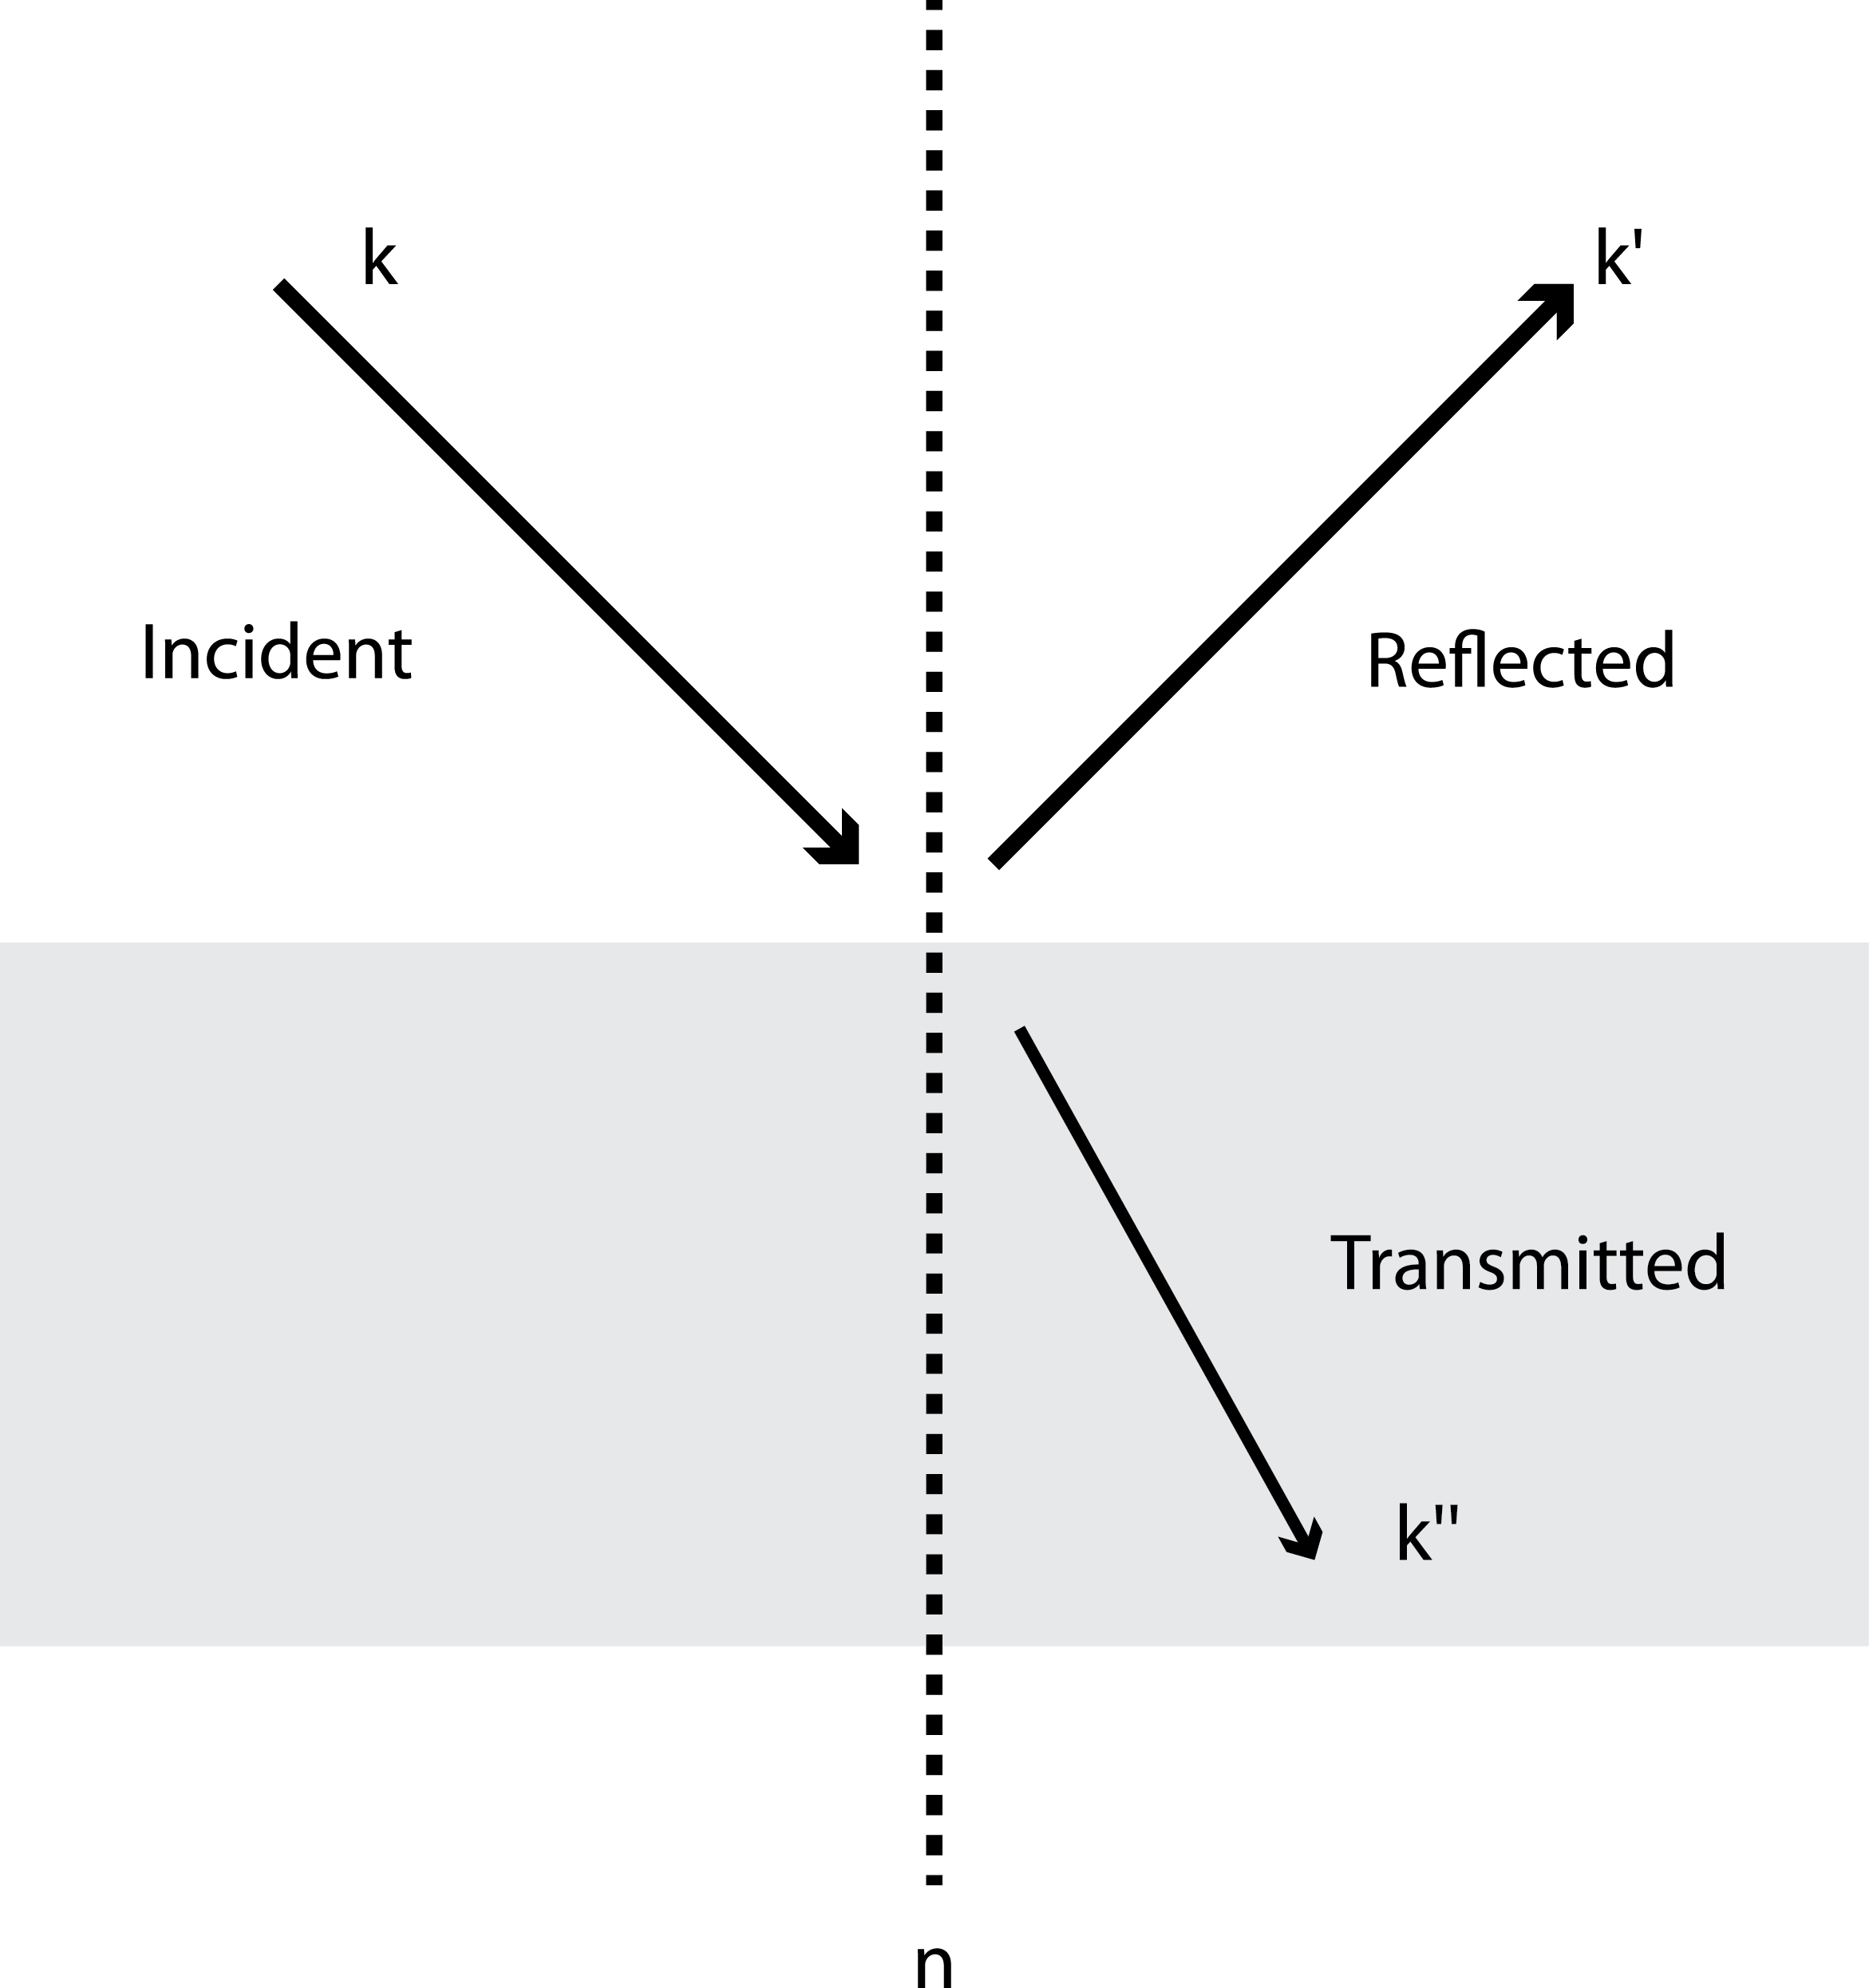
\includegraphics[width=0.6\linewidth, height=0.4\textheight]{Untitled-1}
\caption{Wave vectors for light incident on a boundary separating two different optical media}
\label{fig:Untitled-1}
\end{figure}
Consider a plane harmonic wave incident upon a plane boundary separating two different optical media (See Figure 1.2). There will be a reflected wave a transmitted wave. The space-time dependence of these three waves, aside from constant amplitude factors, is given by the following complex expressions:\\\\
$\exp i(k\cdot r-\omega t)$ incident wave\\
$\exp i(k^{\prime}\cdot r -\omega t)$ reflected wave\\
$\exp i(k^{\prime\prime}\cdot r - \omega t)$ transmitted (refracted) wave\\\\
Now, in order that any constant relation can exist for all points of the boundary and for all values of $t$, it is necessary that the arguments of the three exponential functions be equal at the boundary. Therefore, since the time factors are aşready equal, we will have
\begin{center}
	$k\cdot r=k^{\prime}\cdot r=k^{\prime\prime}\cdot r$ (at boundary)
\end{center}
These equations imply that all three wave vectors $k$, $k^{\prime}$ and $k^{\prime\prime}$ are coplanar, and that their projections onto the boundary plane are all equal. 





















































\chapter{Data and Results}
\begin{table}[h]
	\begin{center}
\begin{tabular}{|c||c|c|c|c|c|c|c|}
	\hline $\theta_{i}$ & 20$^{\circ}$ & 30$^{\circ}$ & 40$^{\circ}$ & 50$^{\circ}$ & 60$^{\circ}$ & 70$^{\circ}$ & 80$^{\circ}$ \\ 
	\hline $\theta_{t}$ & 6$^{\circ}$ & 10$^{\circ}$ & 13$^{\circ}$ & 17$^{\circ}$ & 21$^{\circ}$ & 26$^{\circ}$ & 24$^{\circ}$ \\ 
	\hline 
\end{tabular} 
\end{center}
\caption{Sample data for incidence angle} 
\end{table}
\begin{table}[h]
	\begin{center}
\begin{tabular}{|c||c|c|c|c|c|c|c|c|c|c|c|c|c|}
	\hline $\theta_{i}$ & $20^{\circ}$ & $25^{\circ}$ & $30^{\circ}$ & $35^{\circ}$ & $40^{\circ}$ & $45^{\circ}$ & $50^{\circ}$ & $55^{\circ}$ & $60^{\circ}$ & $65^{\circ}$ & $70^{\circ}$ & $75^{\circ}$ & $80^{\circ}$ \\ 
	\hline $I(\theta_{i})_{\parallel}$ & $28^{\circ}$ & $26^{\circ}$ & $23^{\circ}$ & $17^{\circ}$ & $14^{\circ}$ & $8^{\circ}$ & $4^{\circ}$ & $4^{\circ}$ & $6^{\circ}$ & $14^{\circ}$ & $15^{\circ}$ & $20^{\circ}$ & $32^{\circ}$ \\ 
	\hline 
\end{tabular} 
\end{center}
\caption{Sample data for parallel intensity} 
\end{table}
\begin{table}[h]
	\begin{center}
		\begin{tabular}{|c||c|c|c|c|c|c|c|c|c|c|c|c|c|}
			\hline $\theta_{i}$ & $20^{\circ}$ & $25^{\circ}$ & $30^{\circ}$ & $35^{\circ}$ & $40^{\circ}$ & $45^{\circ}$ & $50^{\circ}$ & $55^{\circ}$ & $60^{\circ}$ & $65^{\circ}$ & $70^{\circ}$ & $75^{\circ}$ & $80^{\circ}$ \\ 
			\hline $I(\theta_{i})_{\perp}$ & $26^{\circ}$ & $24^{\circ}$ & $22^{\circ}$ & $16^{\circ}$ & $13^{\circ}$ & $8^{\circ}$ & $4^{\circ}$ & $3^{\circ}$ & $6^{\circ}$ & $18^{\circ}$ & $16^{\circ}$ & $25^{\circ}$ & $29^{\circ}$ \\ 
			\hline 
		\end{tabular} 
	\end{center}
	\caption{Sample data for perpendicular intensity} 
\end{table}
\textbf{1. Referring the Table 2.1, plot $\sin\theta_{i}$ versus $\sin\theta_{t}$. From the slope of this graph determine the refractive index $n_{2}$ of the cylindrical block of material.} \textit{Note: While plotting the trendline of the graph by using MS Excel$^{\textregistered}$, use linear type and specify the equation of trendline.}
\begin{figure}[h!]
\centering
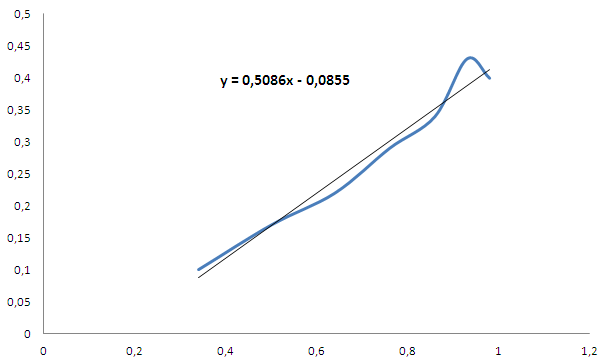
\includegraphics[width=1.0\linewidth, height=0.4\textheight]{g1}
\caption{$\sin\theta_{i}$ vs $\sin\theta_{t}$ graph}
\label{fig:g1}
\end{figure}
\begin{center}
	\begin{tabular}{|c||c|}
	\hline $n_{2}$ & 0.5 \\ 
	\hline 
\end{tabular} 
\end{center}
Slope of the equation is correspond to refractive index $n_{2}$. As we know, in a first degree equation, $y=mx+b$, $m$ is correspond to slope of the equation.\\\\
\textbf{2. Locate the Brewster angle.}
\begin{center}
	\begin{tabular}{|c||c|}
		\hline $\theta_{B}$ & 26.95$^{\circ}$ \\ 
		\hline 
	\end{tabular} 
\end{center}
As we know, the refractive index of air is 1.0 that means $n_{1}=1.0$. Since Brewster Angle $\theta_{B}=\tan^{-1}\frac{n_{2}}{n_{1}}$
\begin{center}
	$\theta_{B}=\tan^{-1}\frac{0.5086}{1.0}=0.5086=26.95^{\circ}$
\end{center}
\textbf{3. Referring Table 2.2 and 2.3, compute the ratio $I_{\parallel}/I_{\perp}$ for the reflected beam and plot this as a function of incident angle, $\theta_{i}$.} \textit{Note: While plotting the trendline of the graph by using MS Excel$^{\textregistered}$, use $4^{\circ}$ Polynomial Type.}\\\\
See Graphs 2.2 and 2.3.\\\\
\begin{figure}[h!]
\centering
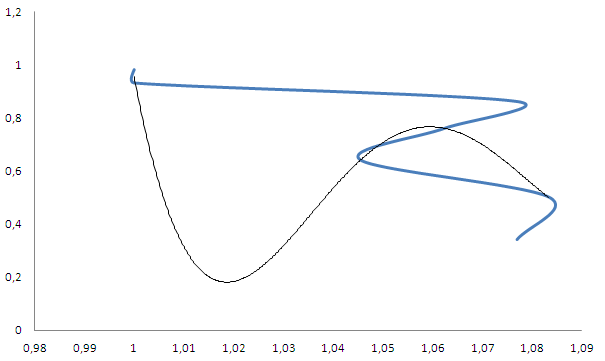
\includegraphics[width=1.0\linewidth, height=0.4\textheight]{g2}
\caption{$[I_{\parallel}/I_{\perp}]$ vs $\theta_{i}$ graph}
\label{fig:g2}
\end{figure}
\begin{figure}[h!]
\centering
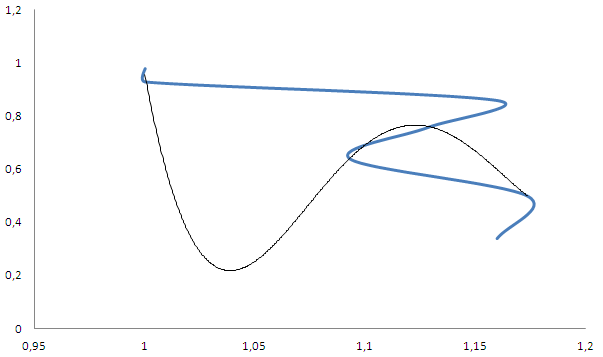
\includegraphics[width=1.0\linewidth, height=0.4\textheight]{g3}
\caption{$[I_{\parallel}/I_{\perp}]^{2}$ vs $\theta_{i}$ graph}
\label{fig:g3}
\end{figure}
\textbf{4. Using $r_{\parallel}=\frac{\tan(\theta_{i}-\tan_{t)}}{\tan(\theta_{i}+\tan_{t)}}$ and $r_{\perp}=\frac{\sin(\theta_{i}-\tan_{t)}}{\sin(\theta_{i}+\tan_{t)}}$, plot theoretical curve $[I_{\parallel}/I_{\perp}]^{2}$ as a function of incident angle, $\theta_{i}$.}\\\\
See Graph 2.4.\\\\
\begin{figure}[h!]
\centering
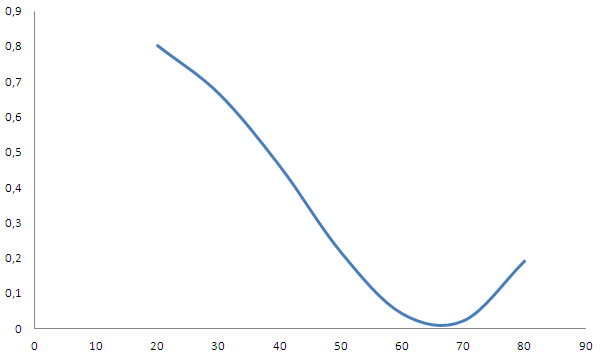
\includegraphics[width=1.0\linewidth, height=0.4\textheight]{g4}
\caption{$[I_{\parallel}/I_{\perp}]^{2}$ vs $\theta_{i}$ graph - Theoretical Value used}
\label{fig:g4}
\end{figure}
\textbf{5. Compare the experimental ($I_{\parallel}/I_{\perp}$ vs $\theta_{i}$) and the theoretical ($[I_{\parallel}/I_{\perp}]^{2}$ vs $\theta_{i}$) curves.}\\\\
Since we did experiment wrongly, we cannot compare theoretical and experimental results. There is an huge difference between them. 







\chapter{Discussion and Conclusion}
\textbf{1.What are the possible errors in the experiment?}\\
Since we did experiment wrongly, we cannot determine the possible errors.\\\\
\textbf{2.What kind of approximation did you take into consideration while you were obtaining the physical quantities and how do they affect your results?}\\
There is no approximation in this experiment.\\\\
\textbf{3.What discrepancies did you encounter between the calculated quantities and theoretical or literature values?}\\
As we mentioned above, we did experiment wrongly. That is why, there are lots of discrepancies between theoretical and experimental values.\\\\
\textbf{4.What is your overall conclusion?}\\
Unlike wrong experimental results, in my opinion, one of the most basic theory of optics which is reflection is studied well in this experiment. Probably, while attending last experiment of the semester and this course, we were lack of concentration that is why we did experiment wrongly except 2.1.
\chapter{Application}
\textbf{Anti-Reflective Coating}\\\\
An antireflective or anti-reflection (AR) coating is a type of optical coating applied to the surface of lenses and other optical elements to reduce reflection. In typical imaging systems, this improves the efficiency since less light is lost. In complex systems such as a telescope, the reduction in reflections also improves the contrast of the image by elimination of stray light. This is especially important in planetary astronomy. In other applications, the primary benefit is the elimination of the reflection itself, such as a coating on eyeglass lenses that makes the eyes of the wearer more visible to others, or a coating to reduce the glint from a covert viewer's binoculars or telescopic sight.\\\\
Many coatings consist of transparent thin film structures with alternating layers of contrasting refractive index. Layer thicknesses are chosen to produce destructive interference in the beams reflected from the interfaces, and constructive interference in the corresponding transmitted beams. This makes the structure's performance change with wavelength and incident angle, so that color effects often appear at oblique angles. A wavelength range must be specified when designing or ordering such coatings, but good performance can often be achieved for a relatively wide range of frequencies: usually a choice of IR, visible, or UV is offered [3].
\chapter{References}
$[1]$ Hecht, E. (2002). \textit{Optics} (4th ed., p. 325). Reading, Mass.: Addison-Wesley.\\
$[2]$ Fowles, G. (1989). \textit{Introduction to Modern Optics} (2nd ed., Dover ed., p. 26). New York: Dover Publications.\\
$[3]$ Gilchrist, A., \& Nobbs, J. (2000). Colorimetry. In J. Lindon, G. Tranter, \& J. Holmes (Eds.), \textit{Encyclopedia of Spectroscopy And Spectrometry} (1st ed., Vol. 1, p. 337). San Diego: Academic Press.
\end{document}          
